\section{The Simulator Fidelity Gap: Game Engines versus Measured Profiles}
\label{sec:gameengine}
The source of the road profiles decides whether simulated training transfers.
Driven by measured profiles, the parametric half-car gives the results of Section~\ref{sec:results}; driven by synthetic ISO~8608 profiles (V9), it still ranks segments ($\rho=$\,\vvVnineRhoWithin) but over-predicts motorway roughness by \vvVnineBiasMotorway\,m/km.
To measure the fidelity gap of game-engine environments, we benchmark a BeamNG.tech~\cite{beamng} corpus: \geTrips{} manually driven trips (\geKm\,km) of \bngCars{} vehicles on \bngMaps{} maps, logging the vehicle's inertial signals and the ray-cast elevation of the road mesh under both wheel paths, from which IRI labels are computed with the same quarter-car algorithm after the smoothing discussed below.
LightGBM trained on it does not transfer to LiRA-CD: its within-route $\rho$ is \vvBcorrRhoWithin{} and its MAE \vvBcorrMaeWithin\,m/km (\vvBrawRhoWithin{} and \vvBrawMaeWithin\,m/km with unsmoothed labels), and its estimates rise steeply with speed on a fixed road (elasticity \vvBcorrElastPooled; further results in Supplement~\ref{S-sec:s_game}).

\begin{figure}[t]
\centering
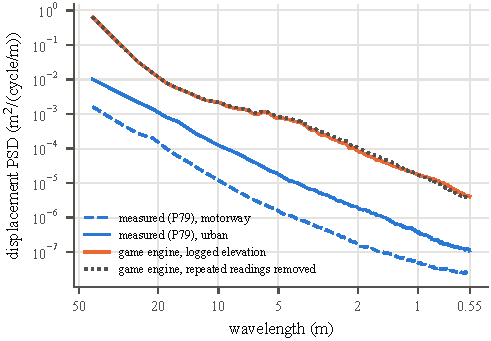
\includegraphics[width=0.8\columnwidth]{v3s_profile_psd.pdf}
\caption{Displacement power spectral density (Welch, detrended, 0.25\,m grid) of the measured P79 profiles (laser 5 and 21) and of the ray-cast mesh elevation of the game-engine corpus (both wheel paths of all trips), as logged and with repeated readings removed.}
\label{fig:profile_psd}
\end{figure}

The ground truth explains much of this.
The ray-cast mesh elevation is far rougher than the measured roads, increasingly so at short wavelengths: its displacement power exceeds that of the urban P79 profiles \gePsdUrbanLong-fold at wavelengths of 10--30\,m and \gePsdUrbanShortMin--\gePsdUrbanShortMax-fold at 0.5--5\,m (Fig.~\ref{fig:profile_psd}), and its IRI averages \geIriLogged\,m/km, against \liraIriUrban\,m/km on the urban P79 roads.
The excess lies in the elevation values, not in their sampling: \geRepeatMin--\geRepeatMax\,\% of the logged readings repeat the previous one while the car moves, but removing the repeats raises the mean IRI to \geIriFresh\,m/km.
A curvature-adaptive smoothing designed to remove mesh tessellation lowers it to \geIriSmoothed\,m/km and changes the condition class of \bngClassChange\,\% of the segments, yet applied to the measured profiles it lowers the urban IRI by \legacyCorrUrbanMape\,\% (Fig.~\ref{S-fig:s_iri}b), so it cannot repair the labels without distorting real roughness.
The logged inertial signals are also degraded: \bngImuDupMin--\bngImuDupMax\,\% of consecutive samples are exact duplicates.
Game engines serve vehicle dynamics and software testing~\cite{gambi2019beamng}, but without measured road profiles they provide neither a valid IRI ground truth nor transferable vibration.
